\documentclass[12pt]{article}
\usepackage{geometry}
\geometry{margin=0.9in}
\usepackage{tikz}
\usepackage{enumitem}
\usepackage{parskip}
\usepackage{xcolor}
\definecolor{isaorange}{HTML}{C2410C}
\definecolor{isagreen}{HTML}{74B566}

\newcommand{\bigtask}[1]{\par\medskip\noindent{\large\textbf{\color{isaorange}#1}}\par}

% A blank hexagon outline for "fill it with triangles".
\newcommand{\hexbox}[1]{%
  \begin{tikzpicture}[scale=#1]
    \draw[line width=1.2pt, isaorange]
      (0:1) -- (60:1) -- (120:1) -- (180:1) -- (240:1) -- (300:1) -- cycle;
  \end{tikzpicture}}

% A blank square for "cut your own tangram / draw a picture".
\newcommand{\squarebox}[1]{%
  \begin{tikzpicture}
    \draw[line width=1.2pt] (0,0) rectangle (#1,#1);
  \end{tikzpicture}}

\begin{document}

\begin{center}
  {\huge\textbf{Pattern Blocks \& Tangrams}}\\[2pt]
  {\large Shapes that fit together}
\end{center}
\vspace{0.3cm}

\bigtask{1. Fill the hexagon}
How many green triangles cover one hexagon? Fill it in, then write the number.
\begin{center}
  \hexbox{2.6}
\end{center}
\noindent It took \underline{\hspace{2cm}} green triangles.\\[4pt]
Can you fill it a \emph{different} way (some triangles, some bigger pieces)?
I found \underline{\hspace{2cm}} different ways.

\bigtask{2. Tile with no gaps}
Keep adding shapes so they cover everything: \textbf{no gaps, no overlaps.}
That is called a \emph{tiling}. Fill this strip with hexagons and triangles:
\begin{center}
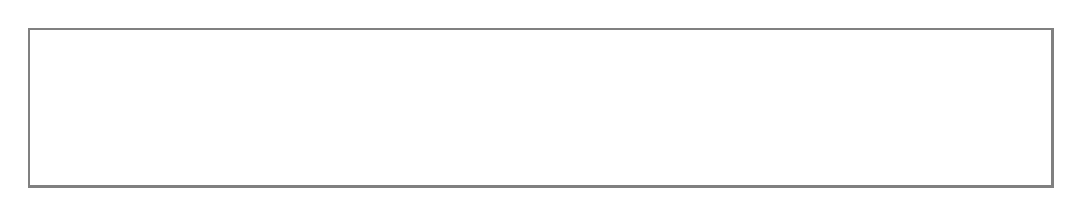
\begin{tikzpicture}
  \draw[line width=1pt, gray] (0,0) rectangle (13,2);
\end{tikzpicture}
\end{center}

\bigtask{3. Which shapes leave a gap?}
Try fitting copies of each shape around one point. Circle the ones that leave a
\textbf{gap} (they will not close up):
\begin{center}
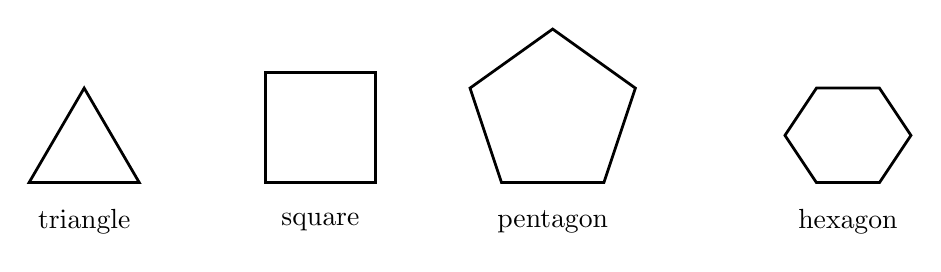
\begin{tikzpicture}[line width=1pt]
  % triangle
  \draw (0,0) -- (1.4,0) -- (0.7,1.2) -- cycle;
  \node at (0.7,-0.5) {triangle};
  % square
  \draw (3,0) rectangle (4.4,1.4);
  \node at (3.7,-0.5) {square};
  % pentagon
  \draw (6.0,0.0) -- (7.3,0.0) -- (7.7,1.2) -- (6.65,1.95) -- (5.6,1.2) -- cycle;
  \node at (6.65,-0.5) {pentagon};
  % hexagon
  \draw (9.6,0.6) -- (10.0,0.0) -- (10.8,0.0) -- (11.2,0.6)
        -- (10.8,1.2) -- (10.0,1.2) -- cycle;
  \node at (10.4,-0.5) {hexagon};
\end{tikzpicture}
\end{center}
\noindent The shape that leaves a gap is the \underline{\hspace{3.5cm}}.

\bigtask{4. Tangram: make a picture}
A tangram is one square cut into \textbf{7} pieces. Use all seven, flat, no
overlaps. Draw a cat, a boat, a rocket, or a person in this box:
\begin{center}
  \squarebox{6}
\end{center}

\end{document}
